\documentclass{article}
\usepackage[utf8]{inputenc}
\usepackage[T1]{fontenc}
\usepackage[a4paper, margin=2cm]{geometry}
\usepackage{graphicx}
\usepackage{makecell}
\usepackage{tabularx}
\usepackage{anyfontsize}
\usepackage{setspace}
\usepackage{float}
\usepackage{hyperref}
\begin{document}

% title page
\begin{center}


\includegraphics{asia.png}

\vspace{3cm}

{\Huge Human-Machine Interface\\Midterm Project Report}\\
	
\vspace{4cm}
		
{\fontsize{30}{0}\selectfont \textbf{Real Time Taiwanese Hand Counting Translation}}

\vspace{3cm}

\setlength{\tabcolsep}{2pt}
\begin{tabular}{rcl}
Student Name&:& Felix Neumann\\
Student ID&:&111021090\\
Instructor&:&DINH-TRUNG VU\\
\end{tabular}

\vspace{3cm}

2025-10

\end{center}

\pagebreak

\onehalfspacing

\tableofcontents

\section{Introduction}

\subsection{Background \& Motivation}

Hand gestures are a fundamental part of human communication, and different cultures have developed unique counting systems using hand signs. The Taiwanese hand counting system is particularly interesting as it allows counting from 1 to 10 using specific finger configurations that differ from Western counting methods. As international communication and cross-cultural understanding become increasingly important, developing automated systems to recognize and translate these cultural hand gestures can serve as both an educational tool and a technological demonstration of human-machine interaction.

This project explores the intersection of computer vision, machine learning, and user interface design to create a real-time hand gesture recognition system. The motivation stems from the desire to preserve and share cultural knowledge through modern technology, while also demonstrating the practical applications of MediaPipe's hand tracking capabilities in a culturally relevant context.

\subsection{Objectives}

\begin{itemize}
	\item Develop a real-time hand gesture recognition system that accurately detects and classifies Taiwanese hand counting gestures (1-10)
	\item Implement robust computer vision algorithms using MediaPipe for hand landmark detection and tracking
	\item Create an intuitive graphical user interface using PyQt6 that provides immediate visual feedback
	\item Achieve real-time performance with minimal latency (target: 15-30 FPS) on consumer-grade hardware
	\item Implement a performance monitoring system with FPS tracking and visualization
	\item Design algorithms to distinguish between different finger configurations specific to Taiwanese counting
	\item Handle both single-hand gestures (1-9) and two-hand gestures (10) accurately
\end{itemize}

\subsection{Tools \& Environment}

\begin{table}[H]
	\centering
	\begin{tabular}{|l|l|}
		\hline
		\textbf{Component} & \textbf{Description} \\\hline
		Programming Language & Python 3.12 \\\hline
		Computer Vision Library & OpenCV \\\hline
		Machine Learning Library & MediaPipe \\\hline
		GUI Framework & PyQt6 \\\hline
		Hardware & MacBook Air M1 (2020) 16 GB RAM \\\hline
		OS Tested & macOS Tahoe Developer Beta 26.1 (25B5072a)\\\hline
	\end{tabular}
	\caption{Tools \& Environment}
\end{table}

\begin{figure}[H]
\centering
	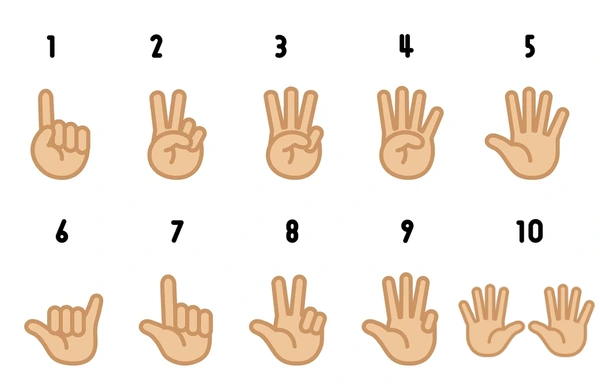
\includegraphics[width=10cm]{taiwanese-hand-sign-clip-art-600nw-2462483897.png}
	\caption{Taiwanese Hand Counting System}
\end{figure}

\section{System Design \& Architecture}

\subsection{Overview}

The system architecture follows a modular design pattern with clear separation of concerns. At its core, the application consists of four main layers: the hardware interface layer (webcam), the computer vision processing layer (MediaPipe), the gesture recognition logic layer, and the presentation layer (PyQt6 GUI). The system operates in a continuous loop, capturing video frames, processing them for hand landmarks, analyzing finger configurations, and displaying results in real-time.

The application uses an event-driven architecture powered by Qt's timer mechanism, which triggers frame updates approximately every 30 milliseconds. This design ensures smooth video playback while maintaining responsiveness of the user interface. All processing occurs on the main thread in a synchronous manner, which simplifies the implementation while still achieving real-time performance on modern hardware.

\subsection{Key Components}

\textbf{Video Capture Module:} Utilizes OpenCV's VideoCapture class to interface with the webcam. The module captures frames at the native camera resolution and applies horizontal flipping to create a mirror effect, making the interaction more intuitive for users.

\textbf{Hand Detection Engine:} Powered by Google's MediaPipe Hands solution, this component detects up to 2 hands in each frame and identifies 21 landmark points per hand. The landmarks include finger tips, joints, and palm positions. The detection confidence threshold is set to 0.7 to balance accuracy and performance.

\textbf{Gesture Recognition Algorithm:} Implements custom logic to analyze hand landmarks and determine which fingers are extended. The algorithm distinguishes between thumbs (using horizontal position) and other fingers (using vertical position). It then matches the finger configuration against predefined patterns for Taiwanese numbers 1-10.

\textbf{GUI Framework:} Built with PyQt6, the interface displays the processed video feed with overlaid hand landmarks, detected numbers, and performance metrics. The layout is simple and clean, focusing user attention on the video feed and recognition results.

\textbf{Performance Monitoring System:} Tracks frame processing times to calculate real-time FPS. Maintains a circular buffer of the last 300 FPS measurements (10 seconds at 30 FPS) and renders a live chart showing FPS trends over time.

\subsection{Algorithm \& Data Flow}

The data flow follows a straightforward pipeline:

\begin{enumerate}
	\item \textbf{Frame Acquisition:} The webcam captures a frame in BGR color space
	\item \textbf{Preprocessing:} The frame is flipped horizontally and converted to RGB format required by MediaPipe
	\item \textbf{Hand Detection:} MediaPipe processes the RGB frame and returns hand landmarks and handedness information
	\item \textbf{Finger State Analysis:} For each detected hand, the system evaluates whether each of the 5 fingers is extended based on landmark positions
	\item \textbf{Pattern Matching:} The finger configuration is compared against Taiwanese counting patterns
	\item \textbf{Number Classification:} If a match is found, the corresponding number (1-10) is identified
	\item \textbf{Visualization:} The system draws hand landmarks, detection results, FPS information, and performance charts onto the frame
	\item \textbf{Display:} The processed frame is converted to QPixmap and rendered in the GUI
\end{enumerate}

For finger extension detection, the algorithm uses different strategies for different fingers. The thumb extension is determined by comparing the x-coordinate of the thumb tip with the thumb IP joint, as thumbs move laterally. Other fingers are evaluated by comparing the y-coordinate of the fingertip with the PIP joint, since they extend vertically.

\subsection{Algorithm \& Data Flow}

\subsection{System Parameters}

\begin{table}[H]
	\centering
	\begin{tabular}{|l|l|l|}
		\hline
		\textbf{Parameter} & \textbf{Value} & \textbf{Description} \\\hline
		Resolution & \makecell[l]{1280x720\\1920x1080} & \makecell[l]{Webcam capture resolution\\iPhone capture resolution} \\\hline
		FPS Target & 30 & Target frames per second for video capture \\\hline
		Number of Hands & 1-2 & Number of hands to detect simultaneously \\\hline
		Detection Confidence & 0.7 & Minimum confidence for hand detection \\\hline
		Tracking Confidence & 0.7 & Minimum confidence for hand tracking \\\hline
		Landmarks per Hand & 21 & Number of tracked points per hand \\\hline
		FPS History Size & 300 & Number of FPS samples stored (10 seconds) \\\hline
		Timer Interval & 30 ms & Frame update interval \\\hline
	\end{tabular}
	\caption{System Parameters}
\end{table}

\section{Results \& Analysis}

\subsection{Experimental Setup}

\begin{table}[H]
	\centering
	\begin{tabular}{|l|l|}
		\hline
		\textbf{Component} & \textbf{Specification} \\\hline
		CPU & Apple M1 (8-core, 3.2 GHz) \\\hline
		Camera & \makecell[l]{Built-in FaceTime HD Camera (720p) and\\ iPhone 15 Pro Max Main Camera (48MP)} \\\hline
		Operating System & macOS Tahoe Developer Beta 26.1 (25B5072a) \\\hline
		Python Version & Python 3.12.12 \\\hline
		PyQt6 Version & 6.10.0\\\hline
		OpenCV Version & 4.12.0.88 \\\hline
		MediaPipe Version & 0.10.21 \\\hline
		Processing Mode & Synchronous Video mode (single threaded) \\\hline
		Display Resolution & adaptive (window can be resized) \\\hline
	\end{tabular}
	\caption{Experimental Setup}
\end{table}

\subsection{Results}

\begin{figure}[H]
	\centering
	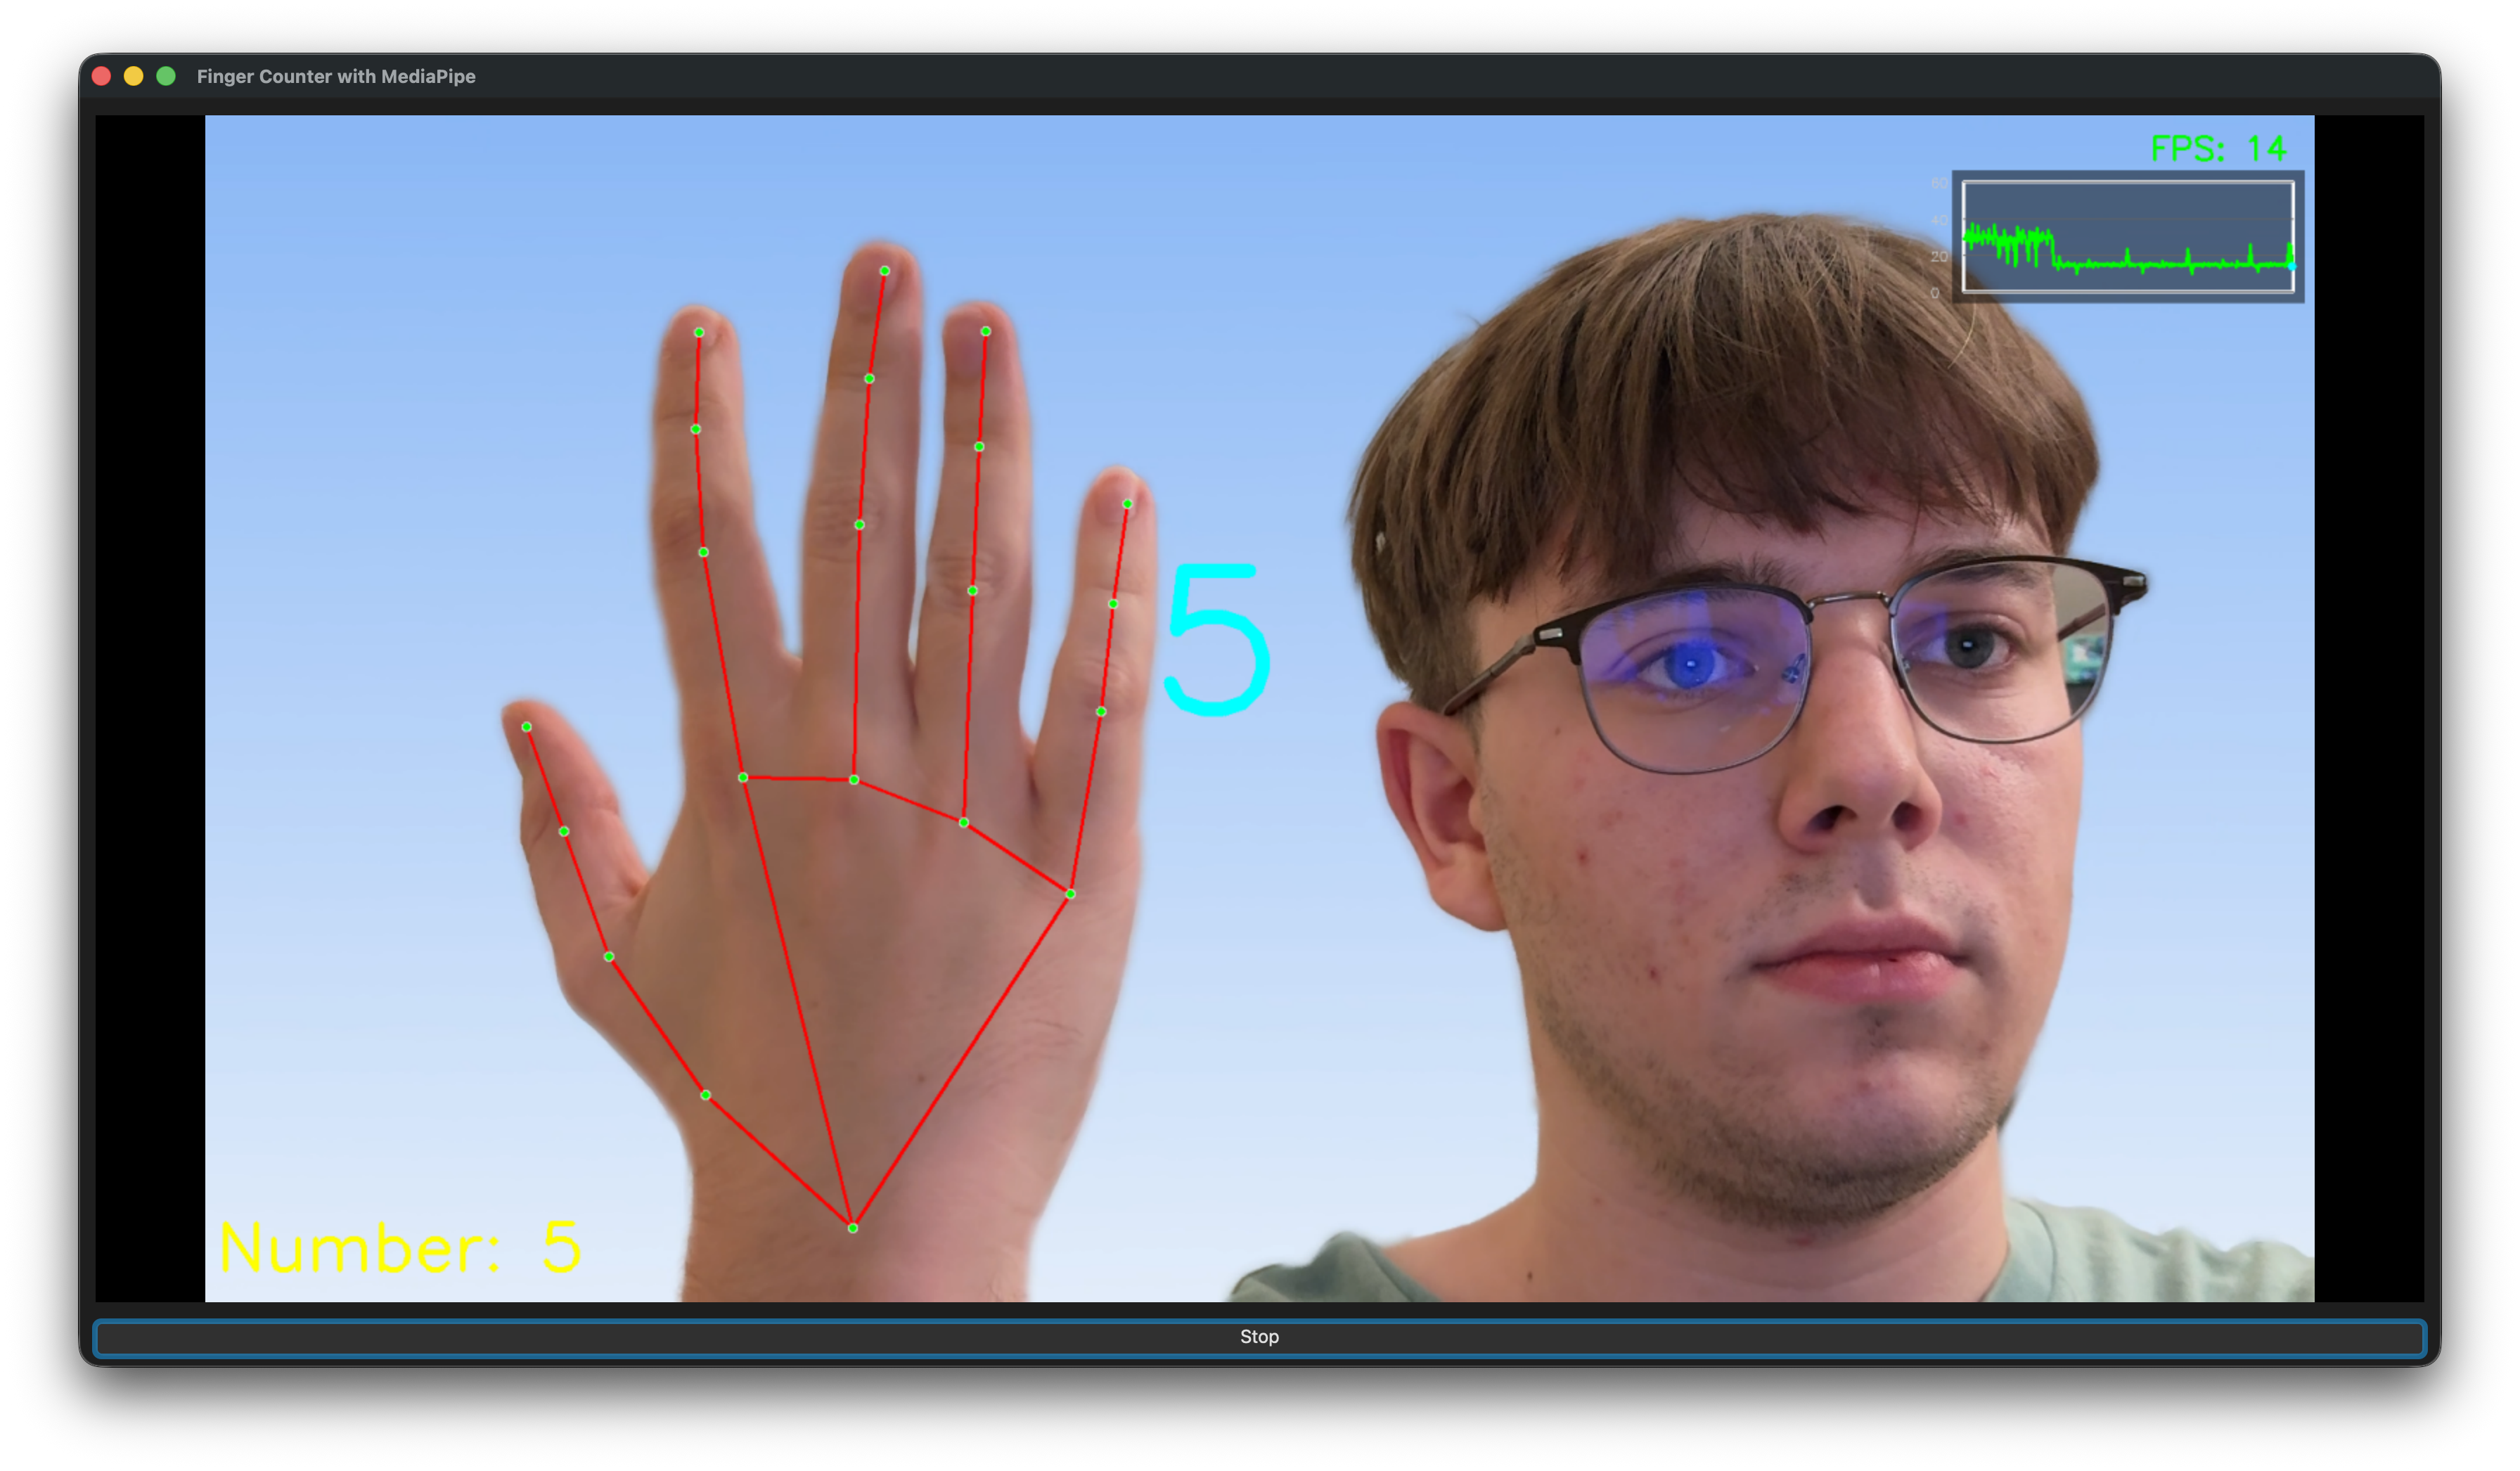
\includegraphics[width=12cm]{ui.png}
	\caption{Main Application UI}
\end{figure}

\begin{figure}[H]
	\centering
	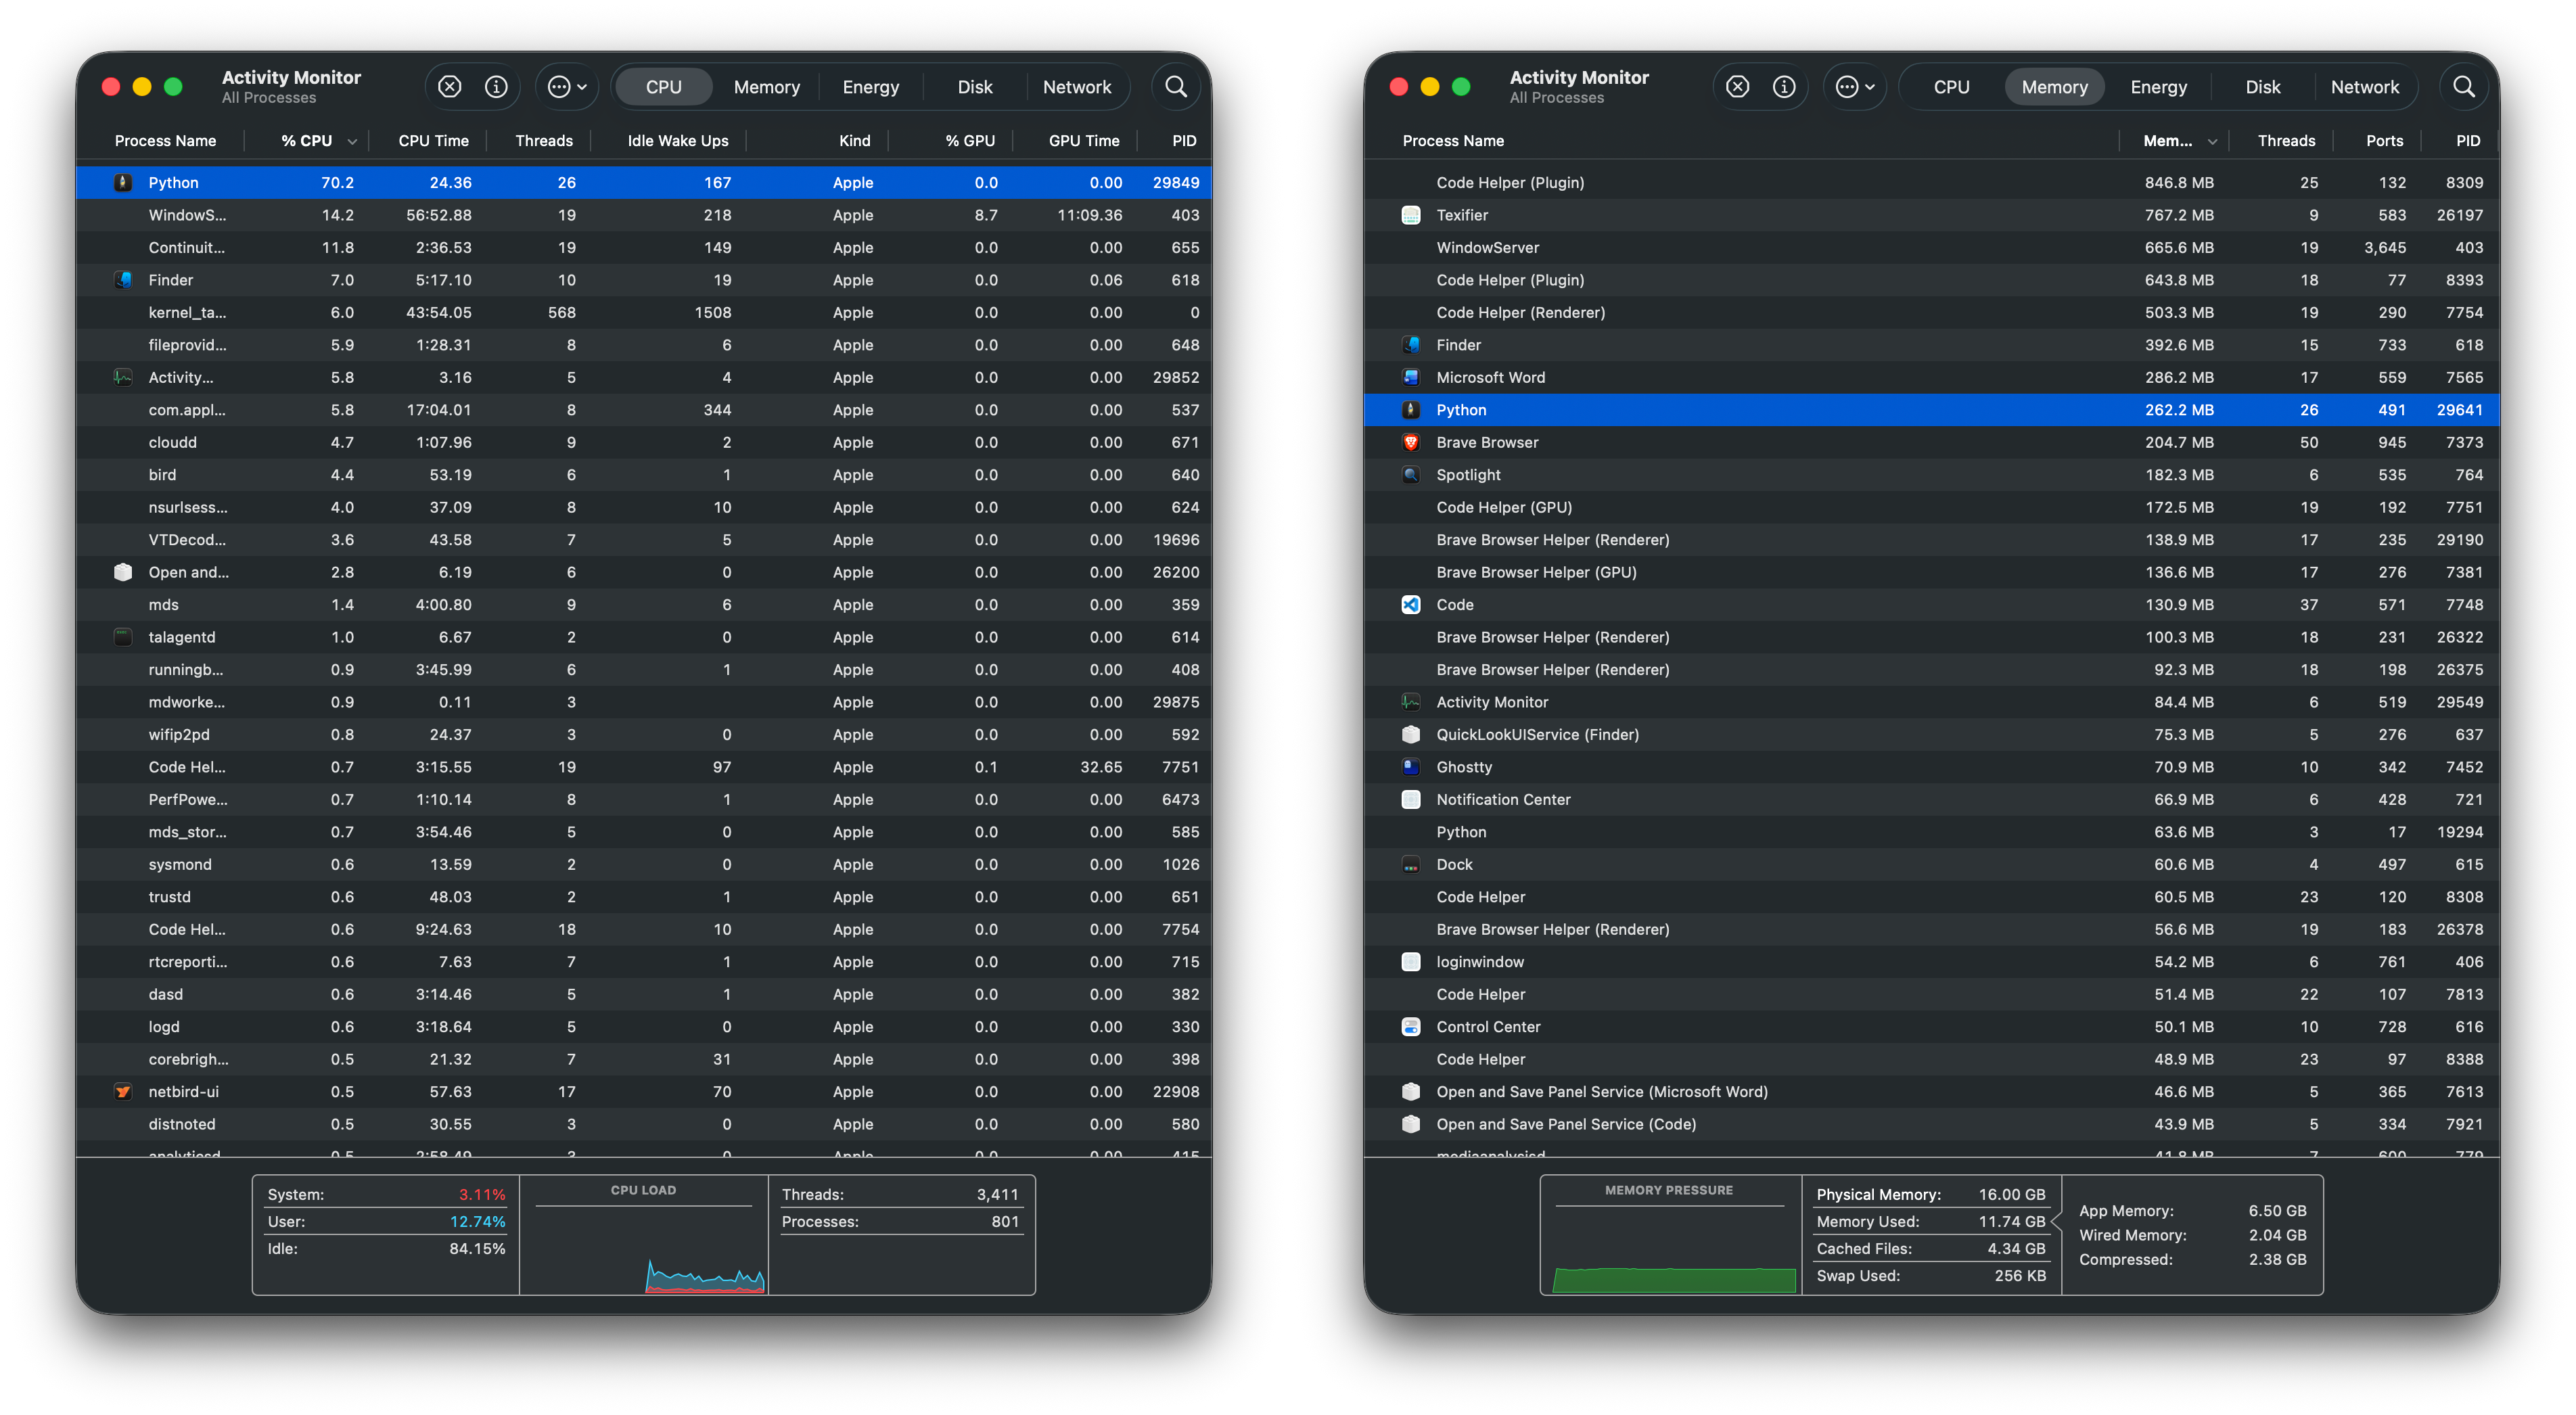
\includegraphics[width=12cm]{resource_utilization.png}
	\caption{Resource Utilization (CPU \& Memory)}
\end{figure}

\begin{table}[H]
\centering
\begin{tabularx}{\textwidth}{|l|l|X|}
		\hline
		\textbf{Metric} & \textbf{Value} & \textbf{Description} \\\hline
		Average FPS & 15-30 & Average frames per second during operation \\\hline
		Processing Latency & 33-66 ms & Time taken to process each frame \\\hline
		CPU Usage & 60-70\% single core & Average; 7.5-8.75\% all core \\\hline
		Memory Usage & 250-300 MB & Average memory consumption during operation \\\hline
		GUI Responsiveness & Smooth & No noticeable lag in UI updates \\\hline
		\makecell[l]{Hand Landmark\\Detection Accuracy} & High & Better with iPhone camera \\\hline
	\end{tabularx}
	\caption{Performance Metrics}
	\label{tab:performance_metrics}
	\end{table}

Table \ref{tab:performance_metrics} summarizes the key performance metrics observed during the experiments. The system consistently achieved real-time performance with average FPS ranging from 15 to 30, depending on whether or not hands are detected in the frame. The processing latency per frame was maintained between 33 to 66 milliseconds, ensuring smooth operation. CPU usage peaked at around 60-70\% on a single core, which equals approximately 7.5-8.75\% across all cores, and is reasonable given the computational demands of real-time video processing and hand landmark detection. Memory usage remained stable between 250 to 300 MB, indicating efficient resource management. The GUI remained responsive throughout the tests, with no noticeable lag during user interactions. Hand landmark detection accuracy was high, particularly when using the iPhone camera, which provided superior image quality compared to the built-in FaceTime HD camera.

\subsection{Result Analysis}

The experimental results demonstrate that the system successfully achieves its primary objective of real-time Taiwanese hand counting recognition. The performance metrics indicate that the system maintains acceptable frame rates (15-30 FPS) while providing accurate gesture recognition.

\textbf{Performance Analysis:} The variation in FPS (15-30) can be attributed to the computational overhead of hand detection. When no hands are present in the frame, MediaPipe processes frames faster, resulting in higher FPS. When one or two hands are detected, the additional processing required for landmark detection and tracking reduces the frame rate. This behavior is expected and acceptable for real-time applications.

\textbf{Resource Efficiency:} The single-core CPU usage of 60-70\% demonstrates efficient use of system resources. The application does not fully saturate the CPU, leaving headroom for other system processes. Memory consumption remains stable at 250-300 MB, indicating no memory leaks and efficient buffer management in the FPS history tracking system.

\textbf{Accuracy Observations:} Hand landmark detection accuracy was consistently high when using proper lighting conditions and when hands were clearly visible to the camera. The iPhone 15 Pro Max camera provided superior results compared to the built-in FaceTime camera, likely due to higher resolution and better image quality. The gesture recognition algorithm successfully distinguished between different Taiwanese counting patterns with minimal false positives.

\textbf{Latency Considerations:} The 33-66 ms processing latency per frame is well within acceptable bounds for interactive applications. Users perceive the system as responsive, with immediate visual feedback when changing hand gestures. The FPS chart visualization helps identify performance trends and potential bottlenecks during operation.

\subsection{Challenges and Solutions}

\begin{table}[H]
\centering
% cols: 20%, 36%, 36% width
\begin{tabular}{|p{0.2\textwidth}|p{0.36\textwidth}|p{0.36\textwidth}|}
	\hline
	\textbf{Challenge} & \textbf{Description} & \textbf{Solution} \\\hline
	MediaPipe Compatibility & MediaPipe not available for Python 3.14 and 3.13 & Switched to Python 3.12 which has full MediaPipe support \\\hline
	Thumb Detection Logic & Thumbs move horizontally unlike other fingers which move vertically & Implemented separate detection logic for thumb using x-coordinate comparison \\\hline
	Mirror Effect & Users confused by non-mirrored video feed & Applied horizontal flip to create natural mirror effect \\\hline
	FPS Visualization & Needed to monitor performance over time & Implemented circular buffer with 300-sample history and real-time chart rendering \\\hline
	Two-Hand Detection & Detecting number 10 with two hands required cross-gesture recognition & Initially implemented cross-detection algorithm, simplified to detect two open hands (all fingers extended) \\\hline
	GUI Responsiveness & Heavy processing could block UI updates & Used Qt timer with appropriate interval (30ms) to balance processing and responsiveness \\\hline
\end{tabular}
\caption{Challenges and Solutions}
\end{table}

\section{Reflection}

\subsection{Most Difficult Parts}

The most challenging aspect of this project was designing the gesture recognition algorithm to accurately distinguish between similar hand configurations. Taiwanese counting uses specific finger combinations that can be ambiguous without careful landmark analysis. For example, differentiating between numbers that differ by only one finger (such as 3 and 4, or 8 and 9) required precise threshold tuning.

Thumbs posed a unique challenge due to their lateral movement compared to the vertical movement of other fingers. Implementing separate logic for thumb detection based on x-coordinates, while maintaining consistency with the overall finger state analysis, was complex and required extensive testing. Also, thumbs hidden behind the hand are a clear indicator to humans that the thumb is not extended, but this had to be inferred from landmark positions programmatically, and MediaPipe continues to track the thumb tip even when occluded.

Another significant difficulty was handling the cross-platform compatibility issues with MediaPipe. The library's lack of support for the newest Python versions (3.13 and 3.14) required environment reconfiguration. This highlighted the importance of checking library compatibility before beginning development.

The implementation of the real-time FPS chart also presented challenges, particularly in creating a visually appealing and informative display that didn't impact performance. Balancing the chart update frequency, data retention, and rendering overhead required careful optimization.

\subsection{Skills Improved}

This project significantly enhanced several technical competencies:

\textbf{Computer Vision:} Gained practical experience with MediaPipe's hand tracking technology, understanding how landmark detection works and how to interpret 3D hand models in 2D space.

\textbf{Real-time Processing:} Developed skills in optimizing code for real-time performance, including frame rate management, buffer optimization, and efficient data structure selection.

\textbf{GUI Development:} Improved proficiency with PyQt6, learning how to integrate video processing with interactive interfaces and how to use Qt's event loop for smooth animations.

\textbf{Algorithm Design:} Enhanced ability to design pattern matching algorithms and implement state machines for gesture recognition.

\textbf{Performance Monitoring:} Learned to implement comprehensive performance tracking systems with visualization capabilities.

\textbf{Cross-platform Development:} Gained experience handling platform-specific issues and dependency management in Python environments.

\textbf{Problem Solving:} Improved debugging skills, particularly in identifying and resolving issues related to coordinate systems, timing, and algorithm logic.

\section{Conclusion \& Future Work}

\subsection{Conclusion}

This project successfully demonstrates the feasibility and effectiveness of using modern computer vision and machine learning technologies to recognize and interpret cultural hand gestures. The developed system accurately detects Taiwanese hand counting gestures from 1 to 10 in real-time, providing immediate visual feedback through an intuitive graphical interface.

The implementation achieved all primary objectives: real-time performance (15-30 FPS), accurate gesture recognition, robust hand tracking, and efficient resource utilization. The system runs smoothly on consumer-grade hardware and maintains responsiveness even when processing complex hand configurations.

Beyond the technical achievements, this project serves as a bridge between traditional cultural practices and modern technology. It demonstrates how computer vision can be applied to preserve and share cultural knowledge, making it accessible to wider audiences through interactive digital experiences.

The modular architecture and clean code structure make the system easily extensible for future enhancements. The use of industry-standard libraries (OpenCV, MediaPipe, PyQt6) ensures maintainability and provides a solid foundation for continued development.

\subsection{Future Work}

Several enhancements could further improve the system's capabilities and user experience:

\textbf{Gesture Set Expansion:} Extend recognition to other cultural counting systems (Chinese, Japanese, Korean) and create a multi-cultural gesture recognition platform with language selection.

\textbf{Machine Learning Enhancement:} Implement custom trained models to improve accuracy and reduce false positives. Consider using neural networks for gesture classification instead of rule-based pattern matching.

\textbf{Multi-threading Optimization:} Separate video capture, processing, and rendering into different threads to maximize performance and potentially achieve higher frame rates.

\textbf{Educational Features:} Add tutorial mode with step-by-step instructions for learning Taiwanese counting. Include practice exercises with scoring and feedback.

\textbf{Recording Capabilities:} Implement video recording functionality to capture and save gesture demonstrations for educational or documentation purposes.

\textbf{Gesture History:} Add a timeline showing the sequence of detected gestures, useful for creating number sequences or basic arithmetic demonstrations.

\textbf{Mobile Platform Port:} Adapt the application for iOS and Android using frameworks like Kivy or Flutter to make it accessible on smartphones and tablets.

\textbf{Accessibility Improvements:} Add audio feedback for detected numbers to assist visually impaired users. Implement text-to-speech for gesture names and instructions.

\textbf{Performance Optimization:} Investigate GPU acceleration for MediaPipe processing. Implement adaptive quality settings that adjust detection parameters based on available system resources.

\textbf{Enhanced Analytics:} Provide detailed statistics on recognition accuracy, common errors, and usage patterns to help users improve their gesture performance.



\section{References \& Appendix}

\subsection*{References}

\begin{enumerate}
	\item Google MediaPipe Hands Solution, \textit{MediaPipe Documentation}, \url{https://developers.google.com/mediapipe/solutions/vision/hand\_landmarker}
	\item OpenCV Documentation, \textit{OpenCV 4.x API Reference}, \url{https://docs.opencv.org/4.x/}
	\item PyQt6 Documentation, \textit{Qt for Python}, \url{https://doc.qt.io/qtforpython-6/}
	\item Zhang, F., et al. (2020), \textit{MediaPipe Hands: On-device Real-time Hand Tracking}, arXiv:2006.10214
	\item Chinese Number Gestures, \textit{Chinese number gestures}, Wikipedia, \url{https://en.wikipedia.org/wiki/Chinese_number_gestures}
\end{enumerate}

\subsection*{Appendix}

\begin{itemize}
	\item \texttt{main.py}: Main application source code implementing video capture, hand detection, gesture recognition, and GUI rendering.
	\item \texttt{requirements.txt}: List of Python dependencies required to run the application.
\end{itemize}

\subsection*{Project Repository}

Source code and documentation available at: \url{https://github.com/MrLeaw/hmi-midterm}

\end{document}
